\newpage

\begin{center}
	\section{Simulaci\'on num\'erica}
\end{center}

\noindent
\justify

El material seleccionado, tanto para el molino como las bolas, es acero es acero A36. Las propiedades del mateial, empleadas para el desarrollo de la simulaci\'on num\'erica, se pueden apreciar en el Cuadro \ref{data}.

\begin{table}[h!]
\centering
\begin{tabular}{c c}
\hline
\textbf{Par\'ametro} &  \textbf{Valor} \\ \hline
Coeficiente de Posisson $(\nu )$ & $0.27$ \\ \hline
Densidad $(\rho )$ & $7850 \left[kg/m^3 \right]$ \\ \hline
M\'odulo de Young $(E )$ & $250 [MPa]$ \\ \hline
Coeficiente de restituci\'on & $0.9$ \\ \hline
Coeficiente de fricci\'on est\'atica $(\mu )$ & $0.15$ \\ \hline
Coeficiente de fricci\'on rotacional & $0.09$ \\ \hline
\end{tabular}
\caption{Propiedades del acero A36.}
\label{data}
\end{table}

\vspace{-0.5cm}

\noindent
\justify

La simulaci\'on se inicia con cuatro tipos de part\'iculas, como se muestra en el Cuadro \ref{particula}.

\begin{table}[h!]
\centering
\begin{adjustbox}{max width=\textwidth}
\begin{tabular}{c c c c c c c}
\hline
\textbf{Di\'ametro} & \textbf{N\degree part\'iculas} & \textbf{Material} & \textbf{Vol. unit. $\left[m^3 \right]$} & \textbf{Masa unit. $[kg]$} & \textbf{Mom. de iner. $\left[kg \, m^2 \right]$\footnote{Por tratarse de cuerpos esf\'ericos, los momentos de inercia en $x$, $y$ y $z$ presentan el mismo valor.}} \\ \hline
$7 [cm]$ & 117 & Acero A36 & $1.79 \, \, 10 ^{-4}$ & $1.41$ & $6.9 \, \, 10 ^{-4}$ \\ \hline
$4 [cm]$ & 627 & Acero A36 & $3.35 \, \, 10^{-5} $ & $0.26$ & $4.16 \, \, 10 ^{-5}$ \\ \hline
$2.5 [cm]$ & 2567 & Acero A36 & $8.18 \, \, 10^{-6}$ & $6.42 \, \, 10^{-2}$ & $4.01 \, \, 10 ^{-6}$ \\ \hline
$100 [\mu m]$ & $102 \, \, 10^9$ & Arena de r\'io & $5.23 \, \, 10^{-13}$ & $7.85 \, \, 10^{-10}$ & $3.14 \, \, 10 ^{-22}$ \\ \hline
\end{tabular}
\end{adjustbox}
\caption{Informaci\'on sobre las part\'iculas de la simulaci\'on.}
\label{particula}
\end{table}

\vspace{-0.5cm}

\noindent
\justify

El objetivo de esta simulaci\'on es encontrar la mejor distribuci\'on de energ\'ia de las bolas sobre el molino variando los siguientes par\'ametros: tama\~no e inclinaci\'on de la aleta, como se muestra en la Figura \ref{aletas}.

\begin{figure}[h!]
\centering
\begin{tikzpicture}
	%Molino
	\draw (-5.2,-0.8) arc(170:10:5.2);
	\draw (-0.81,2.945) arc(-260:-190:5);
	\draw[red] (-0.81,2.945) -- (0,2.2) -- (0.81,2.945);
	\draw (0.81,2.945) arc(80:10:4.8);
	\draw[dotted]  (0.81,2.945) arc(80:90:5);
	
	\draw[dashed, blue] (0,1.4) -- (0,4);
	\draw[arrows={-Triangle[angle=90:5pt,black,fill=black]}] (1.5, 0) -- (1.5,1.8) -- (0.4, 2.52) node[right=1mm] {Aleta};
	
	
	\draw[<-] (0,2.6) arc(90:115:0.8);	
	\node[left] at (-0.05,2.75) {$\theta$};
	
	\draw (0,2.2) -- (-1.2,2.2);
	\draw (0,3) -- (-1.2,3);
	\draw[<-] (-1,3) -- (-1, 2.2);
	\draw[<-] (-1, 2.2) -- (-1,3) node[midway, left=1mm] {$h$};
	
	\draw[blue!50!red, arrows={-Triangle[angle=90:5pt,blue!50!red,fill=blue!50!red]}] (4.8,0.8) arc(20:80:4.5) node [midway, right=0.4mm] {$\overrightarrow{T}$};

	
\end{tikzpicture}
\caption{Geometr\'ia de una aleta.}
\label{aletas}
\end{figure}

\noindent
\justify

De la Figura \ref{aletas}, $h$ es la altura de la aleta y $\theta$ es el \'angulo de inclinaci\'on de la misma, como se aprecia en la Figura.

\subsection{Primera iteraci\'on} \label{primera}

\noindent
\justify

Para la primera iteraci\'on, se emplearon 12 aletas con $h = 30 [mm]$ de altura y $\theta = 45 [\degree ]$ de \'angulo interno (ver Figura \ref{aletas}); bolas de $2.5 [cm]$, $4 [cm]$ y de $7 [cm]$. Al realizar la simulaci\'on num\'erica, se obtuvieron los siguientes resultados:


\begin{figure}[h!]
	\centering
	\begin{subfigure}[b]{0.7\textwidth}
		\centering
		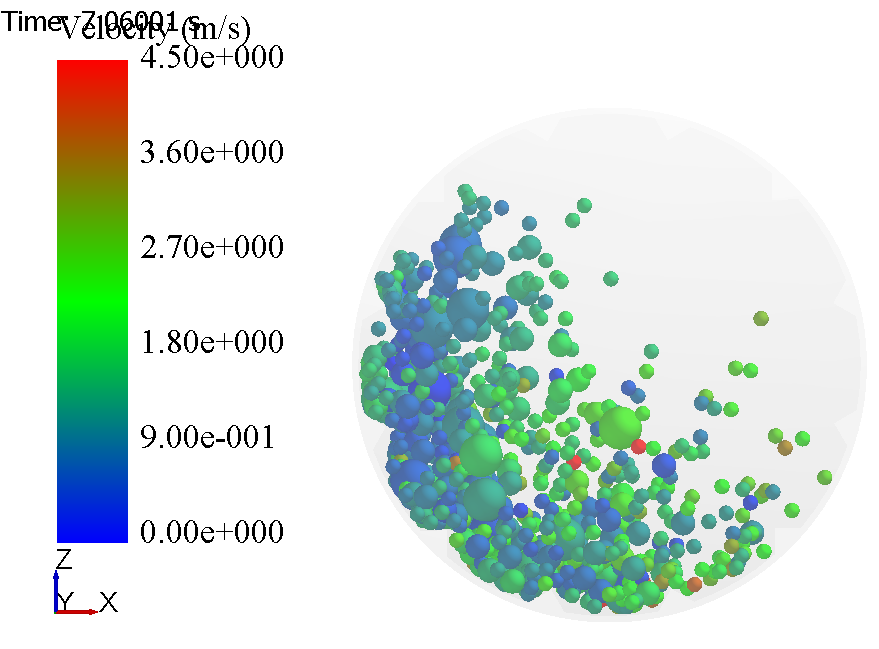
\includegraphics[width=\textwidth]{Images/Resultados/Sim1/sim1.PNG}
		\caption{Perfil de velocidades durante la molienda.}
	\end{subfigure}
	\hfill
	\begin{subfigure}[b]{0.94\textwidth}
		\centering
		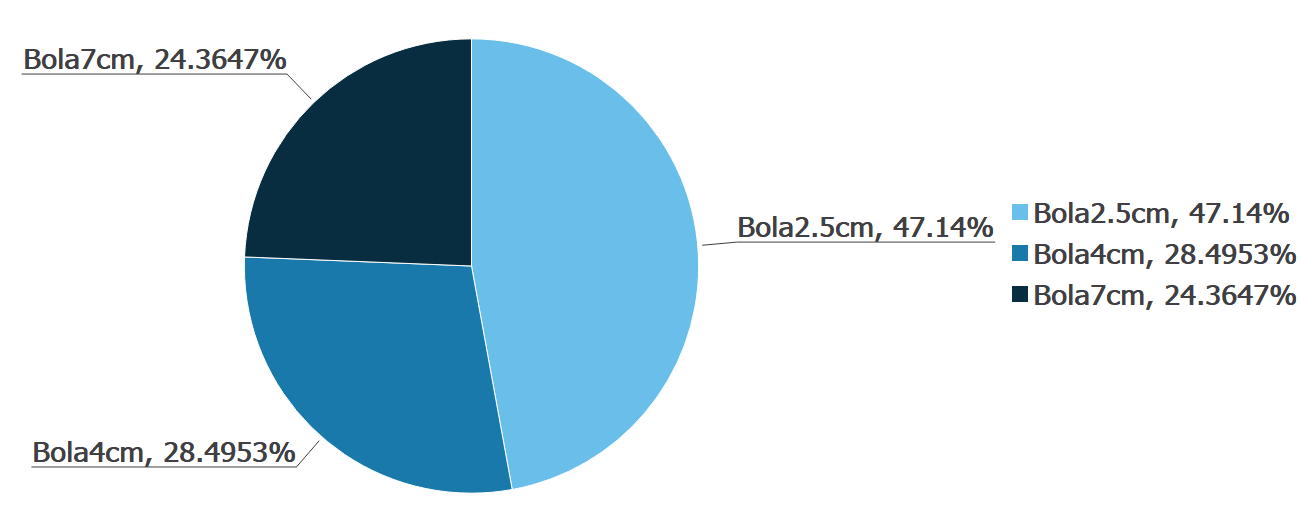
\includegraphics[width=\textwidth]{Images/Resultados/Sim1/dist1.PNG}
	\caption{Distribuci\'on de la energ\'ia de impacto por tipo de bola.}
	\end{subfigure}
	\caption{Resultados iniciales de la primera iteraci\'on.}
	\label{resul1}
\end{figure}


\noindent
\justify

De la Figura \ref{resul1}, se puede apreciar que las esferas de menor di\'ametro $\left( 2.5 [cm] \right)$ tienden a alcanzar velocidades de hasta $4.5 \left[m/s^2 \right]$ de magnitud. La distribuci\'on de la energ\'ia de impacto tiende a ser mayor, para esta configuraci\'on, por parte de las bolas de menor tama\~no con un $47.1 \%$, seguido por las bolas de $4 [cm]$ con un porcentaje del $28.5 \%$ y, finalmente, las bolas de $7 [cm]$, que presentan una distribuci\'on del $24.4 \%$ de la energ\'ia de impacto transmitida.

\begin{figure}[h!]
\centering
\begin{tikzpicture}
	\begin{axis}[grid = both, minor tick num=2,
			title = \textbf{Tiempo vs Energ\'ia cin\'etica},
			xlabel = {Tiempo $[s]$},
			ylabel = {Energ\'ia cin\'etica $[J]$},
			width=\textwidth]
	\addplot[smooth, mark=*, blue!60!black] table [x=TIME, y=E2.5] {Results/res1.txt};
	\addlegendentry{Bolas $2.5 [cm]$}
	\addplot table [x=TIME, y=E4] {Results/res1.txt};
	\addlegendentry{Bolas $4 [cm]$}
	\addplot[smooth, mark=*, green!70!red] table [x=TIME, y=E7] {Results/res1.txt};
	\addlegendentry{Bolas $7 [cm]$}
	\end{axis}
\end{tikzpicture}
\caption{Valor de la energ\'ia cin\'etica m\'axima, por tipo de bola, en el tiempo.}
\label{res1}
\end{figure}

\noindent
\justify

En la Figura \ref{res1}, se observa el valor de la energ\'ia cin\'etica m\'axima, antes de la colisi\'on, d\'onde se observa que la energ\'ia transmitida por las esferas de $7 [cm]$ tiende a ser cerca del doble de las transmitidas por las de $2.5 [cm]$; y que la energ\'ia cin\'etica de las bolas de $2.5 [cm]$ y las de $4 [cm]$ no presenta una diferencia considerable (cerca de $0.5 [J]$ de diferencia).

\noindent
\justify

La etapa de \textit{movimiento parab\'olico} de las bolas dur\'o, en promedio, $0.41 [s]$; arrojando un \textbf{error de simulaci\'on} del $4.65 \%$ (compar\'andolo con el valor de $0.43 [s]$ calculado en la secci\'on \ref{cinema}).

\noindent
\justify

Con base a los resultados mostrados en las Figuras \ref{resul1} y \ref{res1}, se observa que las bolas de $4 [cm]$ no representan un \textit{aporte considerable} en el desempe\~no del molino, por lo que se cambiar\'an por esferas de $5 [cm]$ en futuros an\'alisis.  

\subsection{Segunda iteraci\'on} \label{segunda}

\noindent
\justify

Con base en los resultados obtenidos en la secci\'on \ref{primera}, se realiz\'o una simulaci\'on con los siguientes datos: 10 aletas de $h = 10 [mm]$ y $\theta = 45 [\degree ]$; bolas de $2.5 [cm]$, $5 [cm]$ y $7 [cm]$. Obteniendo los resultados mostrados a continuaci\'on.

\begin{figure}[h!]
	\centering
	\begin{subfigure}[b]{0.66\textwidth}
		\centering
		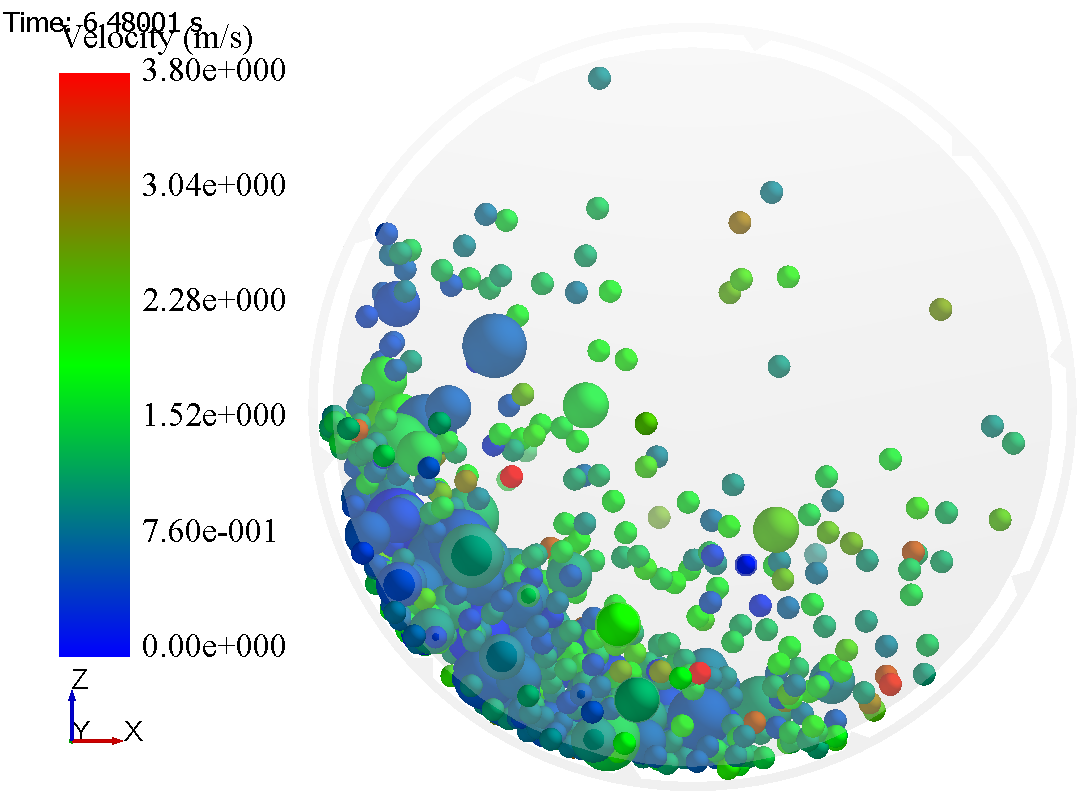
\includegraphics[width=\textwidth]{Images/Resultados/Sim2/sim2.PNG}
		\caption{Perfil de velocidades durante la molienda.}
	\end{subfigure}
	\hfill
	\begin{subfigure}[b]{0.9\textwidth}
		\centering
		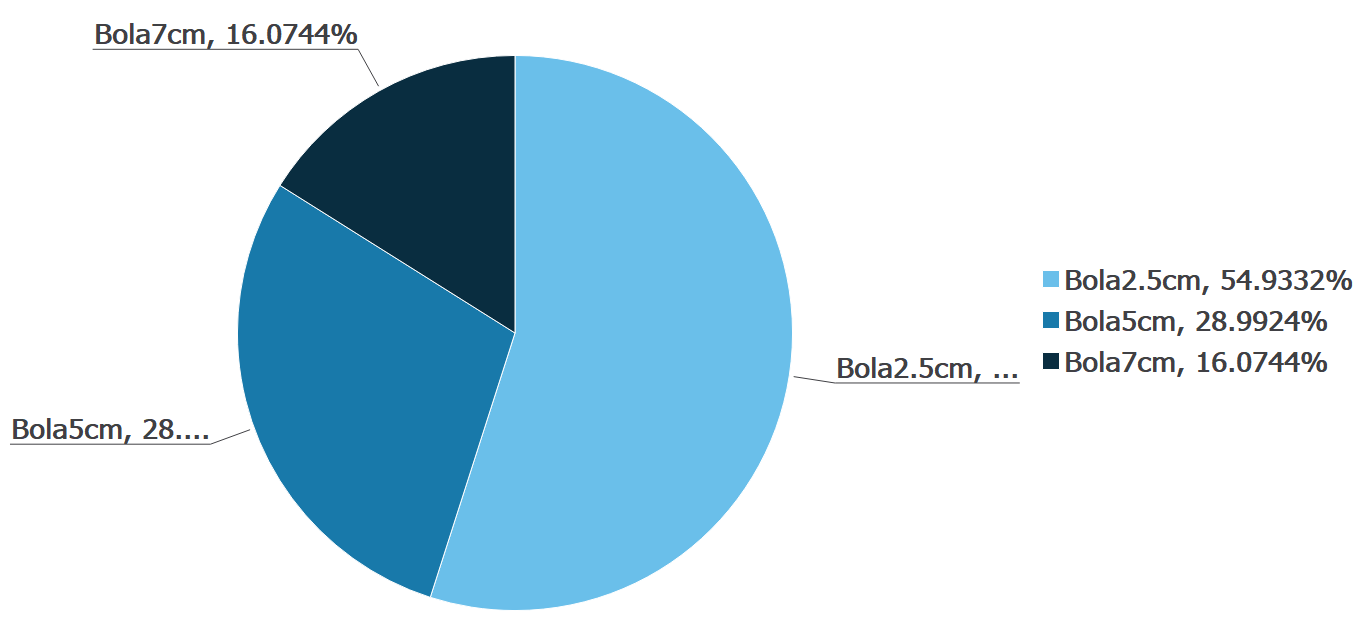
\includegraphics[width=\textwidth]{Images/Resultados/Sim2/dist2.PNG}
	\caption{Distribuci\'on de la energ\'ia de impacto por tipo de bola.}
	\end{subfigure}
	\caption{Resultados iniciales de la segunda iteraci\'on.}
	\label{resul2}
\end{figure}

\noindent
\justify

De la Figura \ref{resul2}, se puede apreciar que las esferas de menor di\'ametro $\left( 2.5 [cm] \right)$ tienden a alcanzar velocidades de hasta $3.8 \left[m/s^2 \right]$ de magnitud. La distribuci\'on de la energ\'ia de impacto tiende a ser mayor, para esta configuraci\'on, por parte de las bolas de menor tama\~no con un $54.93 \%$, seguido por las bolas de $5 [cm]$ con un porcentaje del $28.99 \%$ y, finalmente, las bolas de $7 [cm]$, que presentan una distribuci\'on del $16.07 \%$ de la energ\'ia de impacto transmitida.

\begin{figure}[h!]
\centering
\begin{tikzpicture}
	\begin{axis}[grid = both, minor tick num=2,
			title = \textbf{Tiempo vs Energ\'ia cin\'etica},
			xlabel = {Tiempo $[s]$},
			ylabel = {Energ\'ia cin\'etica $[J]$},
			width=\textwidth]
	\addplot[smooth, mark=*, blue!60!black] table [x=TIME, y=E2.5] {Results/res2.txt};
	\addlegendentry{Bolas $2.5 [cm]$}
	\addplot table [x=TIME, y=E5] {Results/res2.txt};
	\addlegendentry{Bolas $5 [cm]$}
	\addplot[smooth, mark=*, green!70!red] table [x=TIME, y=E7] {Results/res2.txt};
	\addlegendentry{Bolas $7 [cm]$}
	\end{axis}
\end{tikzpicture}
\caption{Valor de la energ\'ia cin\'etica m\'axima, por tipo de bola, en el tiempo.}
\label{res2}
\end{figure}

\noindent
\justify

Al igual que en la Figura \ref{res1}, en la Figura \ref{res2} se observa el valor de la energ\'ia cin\'etica m\'axima antes de la colisi\'on, d\'onde se detalla que la energ\'ia transmitida por las esferas de $7 [cm]$ tiende a ser m\'as del doble de las transmitidas por las de $2.5 [cm]$. A diferencia de la Figura \ref{res1}, la distribuci\'on de la energ\'ia de impacto por tipo de bola es m\'as clara, presentando diferencias apreciables entre s\'i, de m\'as del $50 \%$. Sin embargo, los valores m\'aximos de energ\'ia son significativamente inferiores con esta configuraci\'on; lo que permite concluir que las bolas de $5 [cm]$ confieren mayor eficiencia a la molienda, pero se reduce la efectividad debido a la geometr\'ia de las aletas.

\noindent
\justify

La etapa de \textit{movimiento parab\'olico} de las bolas dur\'o, en promedio, $0.39 [s]$; arrojando un \textbf{error de simulaci\'on} del $9.3 \%$ (compar\'andolo con el valor de $0.43 [s]$ calculado en la secci\'on \ref{cinema}).

\subsection{Tercera iteraci\'on}

\noindent
\justify

Con base en los resultados obtenidos en la secci\'on \ref{segunda}, se desarroll\'o una simulaci\'on con los siguientes par\'ametros: 10 aletas de $h = 40 [mm]$ y $\theta = 30 [\degree ]$; bolas de $7 [cm]$, $5 [cm]$ y $2.5 [cm]$.

\begin{figure}[h!]
	\centering
	\begin{subfigure}[b]{0.66\textwidth}
		\centering
		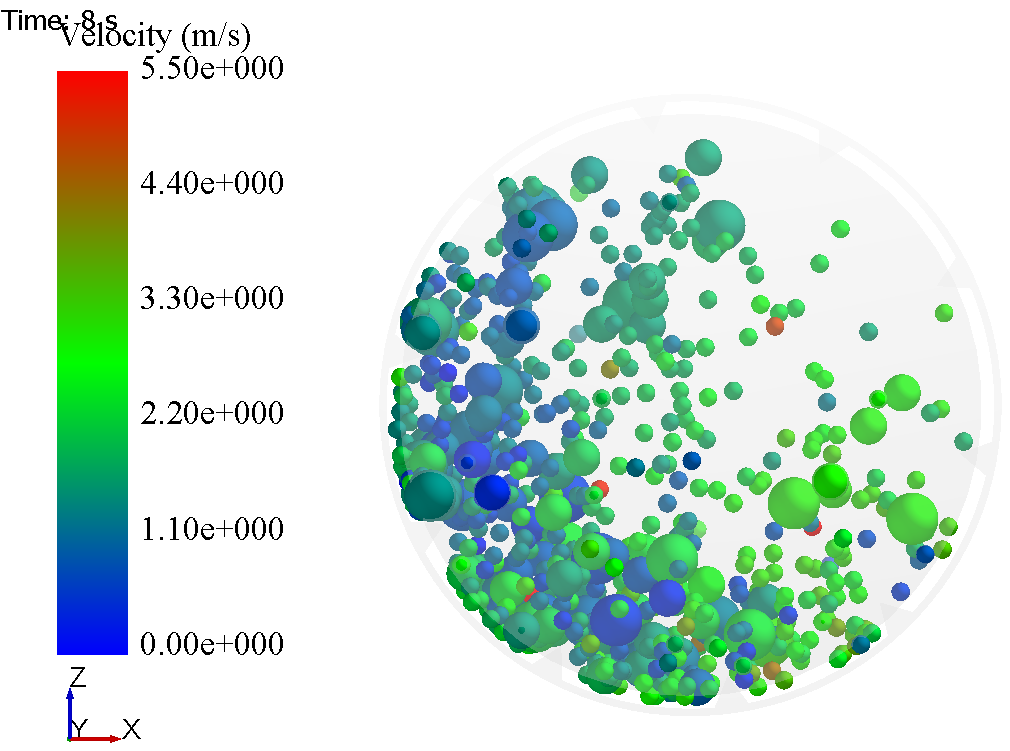
\includegraphics[width=\textwidth]{Images/Resultados/Sim3/sim3.PNG}
		\caption{Perfil de velocidades durante la molienda.}
	\end{subfigure}
	\hfill
	\begin{subfigure}[b]{0.9\textwidth}
		\centering
		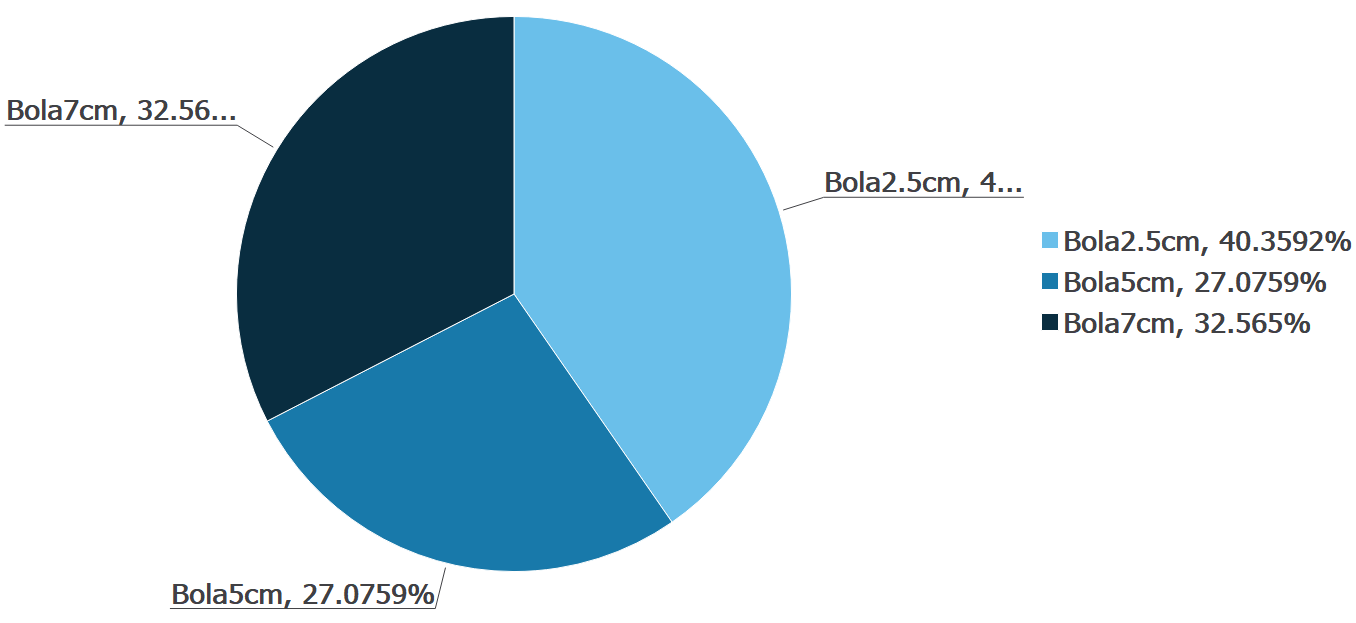
\includegraphics[width=\textwidth]{Images/Resultados/Sim3/dist3.PNG}
	\caption{Distribuci\'on de la energ\'ia de impacto por tipo de bola.}
	\end{subfigure}
	\caption{Resultados iniciales de la tercera iteraci\'on.}
	\label{resul3}
\end{figure}

\noindent
\justify

En la Figura \ref{resul3}, se puede apreciar que las esferas de $2.5 [cm]$ contin\'uan alcanzando las mayores velocidades, llegando con esta configuraci\'on hasta los $5.5 \left[m/s^2 \right]$ de magnitud. La distribuci\'on de la energ\'ia de impacto tiende a ser m\'as equitativa que en las iteraciones anteriores, donde las bolas de menor tama\~no presentan un $40.35 \%$ de distribuci\'on, seguido por las bolas de $7 [cm]$ con un porcentaje del $32.56 \%$ y, finalmente, las bolas de $5 [cm]$, que presentan una distribuci\'on del $27.08 \%$ de la energ\'ia de impacto transmitida.


\begin{figure}[h!]
\centering
\begin{tikzpicture}
	\begin{axis}[grid = both, minor tick num=2,
			title = \textbf{Tiempo vs Energ\'ia cin\'etica},
			xlabel = {Tiempo $[s]$},
			ylabel = {Energ\'ia cin\'etica $[J]$},
			width=\textwidth]
	\addplot[smooth, mark=*, blue!60!black] table [x=TIME, y=E2.5] {Results/res3.txt};
	\addlegendentry{Bolas $2.5 [cm]$}
	\addplot table [x=TIME, y=E5] {Results/res3.txt};
	\addlegendentry{Bolas $5 [cm]$}
	\addplot[smooth, mark=*, green!70!red] table [x=TIME, y=E7] {Results/res3.txt};
	\addlegendentry{Bolas $7 [cm]$}
	\end{axis}
\end{tikzpicture}
\caption{Valor de la energ\'ia cin\'etica m\'axima, por tipo de bola, en el tiempo.}
\label{res3}
\end{figure}

\noindent
\justify

En la Figura \ref{res3}, se aprecia el valor de la energ\'ia cin\'etica m\'axima antes de la colisi\'on. Compar\'andola con los resultados anteriores, se observa una mayor energ\'ia de impacto y una mejor distribuci\'on entre los diferentes tipos de bola, lo que hace de esta alternativa, no s\'olo la m\'as eficiente, sino tambi\'en la m\'as efectiva.

